\documentclass{article}
\usepackage[utf8]{inputenc}
\usepackage[spanish]{babel}
\usepackage{listings}
\usepackage{graphicx}
\graphicspath{ {images/} }
\usepackage{cite}

\begin{document}

\begin{titlepage}
    \begin{center}
        \vspace*{1cm}
            
        \Huge
        \textbf{Proyecto de Investigación}
            
        \vspace{0.5cm}
        \LARGE
        Taller Noción de la memoria del computador
            
        \vspace{1.5cm}
            
        \textbf{Maria Cristina Vergara Quinchia}
            
        \vfill
            
        \vspace{0.8cm}
            
        \Large
        Despartamento de Ingeniería Electrónica y Telecomunicaciones\\
        Universidad de Antioquia\\
        Medellín\\
        Septiembre de 2020
            
    \end{center}
\end{titlepage}

\tableofcontents
\newpage
\section{Introducción}\label{intro}
Esta es la primera sección, podemos agregar algunos elementos adicionales y todo será escrito correctamente. Más aún, si una palabra es demasiado larga y tiene que ser truncada, babel tratará de truncarla correctamente dependiendo del idioma.

\section{Contenido} \label{contenido}
A continuación se desarrollarán los puntos propuestos en el taller 
\subsection{Defina que es la memoria del computador}


\subsection{Mencione los tipos de memoria que conoce y haga una pequeña descripción de cada tipo.}


\subsection{Describa la manera como se gestiona la memoria en un computador}


\subsection{¿Qué hace que una memoria sea más rápida que otra? ¿Por qué esto es importante?}
 \subsection{ Citación}
 
Vamos a citar por ejemplo un artículo de \textbf{Albert Einstein} \cite{einstein}.
También es posible citar libros \cite{dirac} o documentos en línea \cite{knuthwebsite}.

\section{Imágenes} \label{imagenes}

En la Figura (\ref{fig:memoria}), se puede observar una memoria RAM

\begin{figure}[h]
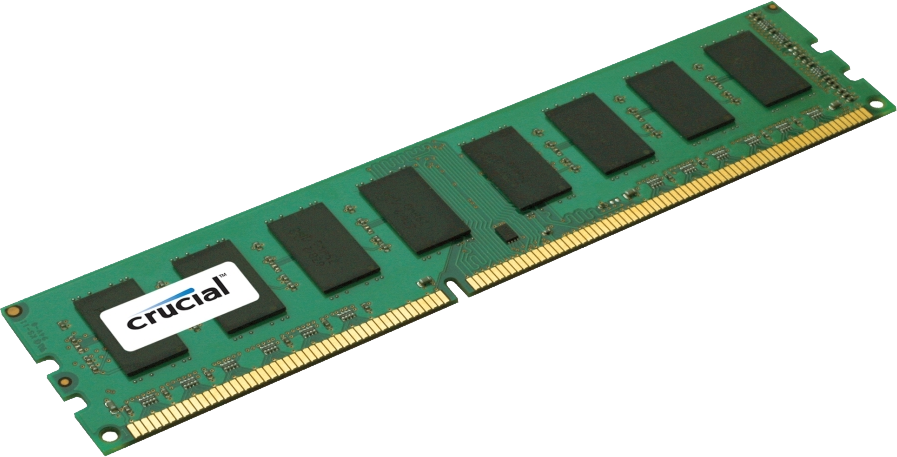
\includegraphics[width=4cm]{memoria.png}
\centering
\caption{Memoria RAM}
\label{fig:memoria}
\end{figure}

Las secciones (\ref{intro}), (\ref{contenido}) y (\ref{imagenes}) dependen del estilo del documento.
\newpage
\bibliographystyle{IEEEtran}
\bibliography{references}

\end{document}
